

\documentclass[table]{sig-alternate-05-2015}


\usepackage{pgf}
\usepackage{tikz}
\usepackage{subcaption}
\usepackage{xcolor}
\usepackage{graphicx}

\usetikzlibrary{arrows,automata}

\begin{document}

% Copyright
%\setcopyright{acmcopyright}
%\setcopyright{acmlicensed}
%\setcopyright{rightsretained}
%\setcopyright{usgov}
%\setcopyright{usgovmixed}
%\setcopyright{cagov}
%\setcopyright{cagovmixed}


% DOI
%\doi{10.475/123_4}
%
%% ISBN
%\isbn{123-4567-24-567/08/06}
%
%%Conference
%\conferenceinfo{PLDI '13}{June 16--19, 2013, Seattle, WA, USA}
%
%\acmPrice{\$15.00}

%
% --- Author Metadata here ---
\conferenceinfo{IntSim}{2015, Augsburg}
%\CopyrightYear{2007} % Allows default copyright year (20XX) to be over-ridden - IF NEED BE.
%\crdata{0-12345-67-8/90/01}  % Allows default copyright data (0-89791-88-6/97/05) to be over-ridden - IF NEED BE.
% --- End of Author Metadata ---

\title{An Interactive Simulation on Spreading of Diseases by Infrastructure}

\numberofauthors{1} %  in this sample file, there are a *total*

\author{

\alignauthor
Patrick Blickling and Philipp Mascha\\
       \affaddr{University of Augsburg}\\
       \email{patrick.blickling@hotmail.de, p.mascha@gmx.net}
       }


\maketitle


\begin{abstract}
We provide an interactive, real-time simulation featuring a large group of self-organized agents in a virtual environment resembling a city. These agents may get infected by diseases or spread them to others by different means of contagion.

The user has to try to contain disease spread by changing the city's infrastructure, building check-points, block roads or build new ones. At the same time, he has to keep the population happy by retaining access to all vital points of interest.

Our simulation features different levels which differ by forms of disease spreading and means off traffic control available. Additionally, we provide a sophisticated agent model with self-learning capabilities.

The goal of our work is to help an user understand the impact of structural changes on disease spreading, as well as an idea on how to contain epidemics.
\end{abstract}

\section{Introduction}
%\begin{itemize}
%\item introduce the general topic
%\item introduce to your idea and your methodology
%\item in this context you conclude the introduction with an outline of the remainder of the paper, e.g. ``[...] in Section 2, we provide a brief survey on related work around developmental systems and interactive art installations. Section 3 presents...''
%\end{itemize}

Great epidemics always have and will embody a great threat to humanity. Pandemics like the Black-Death, viruses like HIV and even the Flu have cost many lives in human history or even whipped out whole civilizations.

While epidemics have been part of our environment more or less all the time, we're still not capable to cope with them adequately. Missing education seems to be the main reason why viruses like HIV are still huge problems in a large part of the world and even plagues like the Black-Death are re-conquering their ground - even in advanced cultures like the US \footnote{\url{www.cdc.gov/plague/maps/}}.

Also, the recent outbreak of Ebola in 2014 showed how important infrastructure is for the spreading of diseases\footnote{\url{en.wikipedia.org/wiki/Ebola_virus_epidemic_in_West_Africa}, invoked on January the 16, 2016}. While originating in Guinea, the epidemic made use of out vast network of globalized transportation, covering not even large parts of Africa but spreading even to remote countries like the US or the United Kingdom in the process. Closing of borders and trastic reduction of tourism was the consequence, resulting in huge economical drawbacks in the affected countries\footnote{\url{www.undp.org/content/undp/en/home/presscenter/pressreleases/2015/03/12/west-african-economies-feeling-ripple-effects-of-ebola-says-un.html}}.

This is why we propose an interactive simulation to show the spreading of various diseases. We aim not to create a completely accurate simulation, both in modeling the diseases as well as in simulating relevant human interaction (tourism, medical research, health-care systems, education \dots). Our first and foremost goal is for the user to grasp the concepts why and how epidemics spread and how adjusted infrastructure can be used to contain these.

\section{Related Work}

Since the topic of disease spread is a vital one, there already exists a vast amount of simulations. These are ranging from very abstract and minimalistic models that only feature the most basic concepts of spread \footnote{\url{www.shodor.org/interactivate/activities/SpreadofDisease/}} to highly sophisticated ones like Biowar \cite{biowar}.

The latter includes a complex agent model based on finite state machines modeling social interactions, daily routines and knowledge transfer. It also considers various environmental parameters like weather or infrastructure. The whole model is based on huge amounts of empirical data, like actual city maps, surveys on various social aspects as well as data about more than 30 diseases.

It's goal is to emulate a real-world scenario as precise as possible to enable predictions when a epidemic may occur or an attack by biological warfare is at hand (hence the name). Our approach differs mainly in these goals: We want to gain more knowledge on how to prevent and contain epidemics rather than foreseeing them. Thus we haven't put our main effort into imitating a specific scenario or city but rather towards creating an interactive simulation that makes the user grasp the inner logic of disease spread.

Since this understanding defines our main design goal, gamification was a important factor to greatly increase user immersion and involvement. Also, instead of basing our agent model on empirical data we decided to use a highly advanced approach using a Learning Classifier System with self-learning capabilities.

There are also games concerning the topic of disease spread like Plague: Inc\footnote{\url{www.ndemiccreations.com/en/22-plague-inc}} or the board game Pandemic. These focus on gamification even more. In the case of Plague:Inc, the user takes the side of the disease and tries to overthrow humanity. It should be obvious that this design goal differs greatly from our work.

\clearpage

%\begin{itemize}
%\item comprehensive background survey
%\item explanations of the related methodologies
%\item summaries of their achievements and their shortcomings
%\item references to seminal publications
%\item how did other works inform yours?
%\item what are those other works about?
%\item how is your work related to other works?
%\item important: what is different?
%\end{itemize}

\section{Models and Methods}

In the following section, we describe how the simulation and its models are designed. User experience, methods of interactions and gamification aspects are emphasized as well as the used models for agents or diseases.

\subsection{General Flow}

\begin{figure}[h]
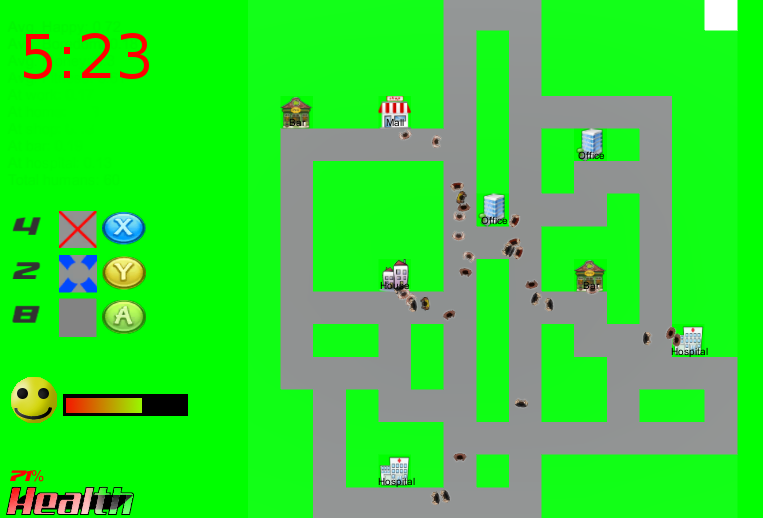
\includegraphics[width = 0.48\textwidth]{Pictures/screen.png}
\caption{A typical simulation screen}
\label{pic:screen}
\end{figure}

When starting the simulation, the user can see the simple layout of a city from a top down view (cf. Fig. \ref{pic:screen}). There are different buildings like offices, hospitals or shops as well as an already existing network of streets. Also, there are people in the city following their every day live, going from one building to another, spending time at each of the different building types.

The user can build new streets or erect checkpoints or blockades that change the routes of the inhabitants. After a short period of time, one or more citizens get infected with a disease. This disease may spread to others under certain conditions.

The task for the user is to keep the number of infected at a minimum. To do this, he has to cleverly place the various infrastructural elements to keep diseased people coming into contact with healthy ones.


\subsection{Win and Lose Conditions}

Our simulation offers multiple levels to the user, which increase in difficulty over their iterations. Each level consists of a unique city layout and a different disease. The different aspects in which diseases may differ are described in section \ref{sec:diseases}.

Also, each level features a certain happiness and infection rate threshold which get narrower with each iteration. The goal for the use is to keep both happiness over and infection rate under these values. If he is able to keep these conditions satisfied for a specific amount of time (which is also level dependent) he may progress to the next level. Otherwise he is triggering a \textit{lose} condition and has to try the current level over.

Each level also features a certain pool of tiles the user may place at maximum. This prohibits the user from using his assets unthoughtful and simulating the restricted budget such emergency situations often have to work with. The amount of tiles the user is allowed to use also decreases over time.

\newpage

\subsection{Interface and Representation}


The main portion of the screen is occupied by the representation of the city. This representation is sectionalized into rectangular tiles containing either streets, buildings or grass. There are 5 types of buildings, as depicted in figure \ref{fig:buildings}.


\begin{figure}[h]
\begin{subfigure}{0.22\textwidth}
\begin{center}

\includegraphics[height = 40pt]{Pictures/Home.png}
\caption{A house providing sleep}
\end{center}
\end{subfigure}
\begin{subfigure}{0.22\textwidth}
\begin{center}
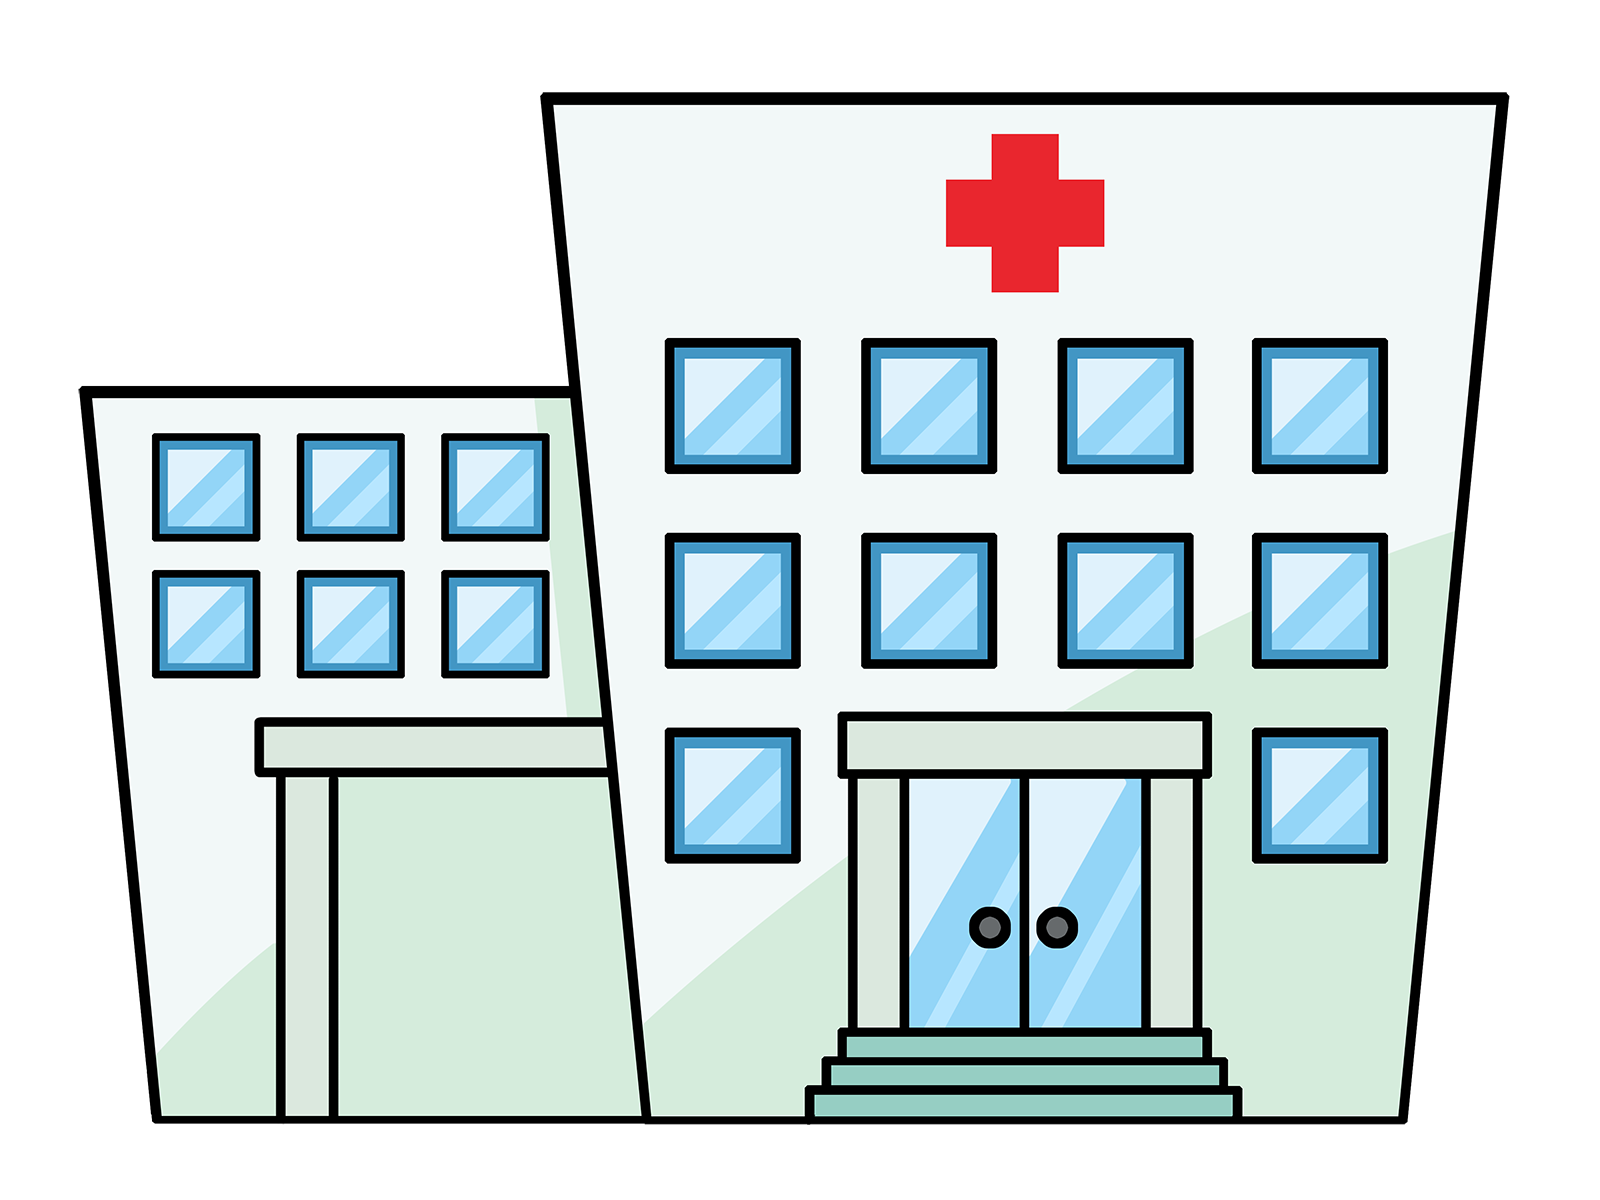
\includegraphics[height = 40pt]{Pictures/Hospital.png}
\caption{A hospital providing health care}
\end{center}
\end{subfigure}
\begin{subfigure}{0.22\textwidth}
\begin{center}

\includegraphics[height =40pt]{Pictures/Office.png}
\caption{Office were citizen can work and earn money}
\end{center}
\end{subfigure}
\begin{subfigure}{0.22\textwidth}
\begin{center}

\includegraphics[height =40pt]{Pictures/Bar.png}
\caption{Bars were citizen find leisure in exchange for money}
\end{center}
\end{subfigure}
\begin{subfigure}{0.22\textwidth}
\begin{center}

\includegraphics[height =40pt]{Pictures/Shop.png}
\caption{A shop providing distraction in exchange for money}
\end{center}
\end{subfigure}
\caption{The different buildings in the city}
\label{fig:buildings}
\end{figure}

\begin{figure}[h]
\begin{center}
\begin{subfigure}{0.2\textwidth}
\begin{center}

\includegraphics[height = 20pt]{Pictures/gui_happy.png}
\caption{The average health, displayed both as bar and numeric value.}
\end{center}
\end{subfigure}
\begin{subfigure}{0.2\textwidth}
\begin{center}

\includegraphics[height = 20pt]{Pictures/gui_health.png}
\caption{The average happiness. If the bar is empty, the level is lost.}
\end{center}
\end{subfigure}
%\caption{Featured tiles}
\caption{GUI elements that inform about the current state of the population.}
\label{fig:gui_bars}
\end{center}
\end{figure}

On the left, important information is displayed, like rate of infection, tiles left to place from the tile pool or the average happiness of the population. Figure \ref{gui_bars} shows these elements. Also, the time left until the current level is finished is displayed on the top left corner.

Citizens are moving on the streets of the city. These aren't bound to the tile grid but can only move on certain tiles, e.g. streets. They may enter or leave buildings. While inside a structure, a citizen isn't displayed on the map. People can't be controlled directly but follow their own decisions and routines, which are described in-depth in section \ref{sec:agents}. 

Despite having no means of direct control, citizens react to changes made to tiles. For example, when a blockade is placed, they will search for another way to reach a certain building. If they can't reach the desired target, they will wait, creating discontent in the process.

\subsection{Controls and Manipulating Infrastructure}
\label{sec:infra}



\begin{figure}[h]
\begin{center}
\begin{subfigure}{0.4\textwidth}
\begin{center}

\includegraphics[width = 50pt]{Pictures/tile_street.jpg}
\caption{Street tiles: These are walkable by all agents.}
\end{center}
\end{subfigure}
\begin{subfigure}{0.4\textwidth}
\begin{center}

\includegraphics[width = 50pt]{Pictures/tile_checkpoint.jpg}
\caption{Checkpoints: These can only be passed by agents without an infection.}
\end{center}
\end{subfigure}
\begin{subfigure}{0.4\textwidth}
\begin{center}

\includegraphics[width =50pt]{Pictures/tile_blockade.jpg}
\caption{Grass and blockades: These can't be entered by anyone.}
\end{center}
\end{subfigure}
\caption{Featured tiles the user may place}
\label{fig:tiles}
\end{center}
\end{figure}

Our simulation features three types of tiles, as depicted in figure \ref{fig:tiles}. These tiles can be set using the simulation controls.

These controls are mapped to a game-pad, in our case the XBox 360/ One controller designed by Microsoft. With the control stick, a tile on the city map can be selected, which is highlighted in the process.

\begin{figure}[h]
\begin{center}
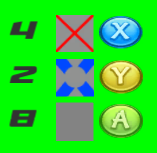
\includegraphics[width = 0.25\textwidth]{Pictures/gui_without_avg.png}
\end{center}
\caption{GUI element to display tiles and their assigned buttons}
\label{pic:gui_tiles}
\end{figure}

By pressing an action button on the pad, the selected tile can be changed to a certain type by pressing an action button on the pad.
Each button is assigned to a specific tile type, as displayed in figure \ref{pic:gui_tiles}, which depicts the corresponding GUI element. The number on the left of each tile displays how many tiles of that specific type are left in the tile pool.

The user may place new streets, blockades and checkpoints at will, but only as much as the current level restrictions allow him to. Each time a new tile is placed, the path-finding of the agents is updated using the shortest-path algorithm by Floyd \cite{floyd}.

\subsection{Diseases and Spreading}
\label{sec:diseases}

In our simulation, there exists two types of important objects: Citizens, henceforth labeled agents, which are described in a later section and disease objects that represent an illness. When a citizen gets infected, an instance of such a disease object is copied and attached to the agent.

\begin{figure}[h]
\begin{center}
\begin{subfigure}{0.2\textwidth}
\begin{center}

\includegraphics[width = 50pt]{Pictures/human.png}
\caption{Healthy}
\end{center}
\end{subfigure}
\begin{subfigure}{0.2\textwidth}
\begin{center}

\includegraphics[width = 50pt]{Pictures/infected.png}
\caption{Infected}
\end{center}
\end{subfigure}
%\caption{Featured tiles}
\caption{Visual feedback concerning agent health}
\label{fig:infected}
\end{center}
\end{figure}

Infected people are displayed in such a manner that they are easily distinguishable by the user (cf. Fig. \ref{fig:infected}). Also, infected agents can't pass checkpoints. In later levels, diseases may have incubation time. This means, that upon infection the disease isn't attached to the agent immediately, but after a short period of time. Thus, the agent can't be recognized as infected at start, ignoring checkpoints, healing through hospitals and missing to integrate the infected state into his decision making (cf. section \ref{sec:decisions}).

There are two types of disease spreading, also dependent on the current level: Infection over air or direct contact. The former infects agents when they are close to each other while they walk by. Every step in the simulation, a infection chance is calculated for each agent depending on how close the agent is to other infected. Then, the simulation evaluates if the agent is infected by random, based on this chance.

Infection by contact spreads when both an diseased and healthy agent are at the same building at the same time, e.g. a shop. This rule doesn't apply to the \textit{hospital} and the \textit{home}, were the agents are considered isolated.

To recover from an infection, the only way is to visit a hospital, given the agent has enough money to pay the visit. A system of public health-care is not included in the simulation.

\subsection{Agent Model}
\label{sec:agents}

The inhabitants of the simulated city consist of  two components: An agent object that executes actions and holds information about the current position and status as well as an artificial intelligence which is used to evaluate situations and make decisions about future actions. The following sections will describe these agents and their model of decision making in-depth.

\subsubsection{Regarding Finite State Machines}

\begin{figure}[h]
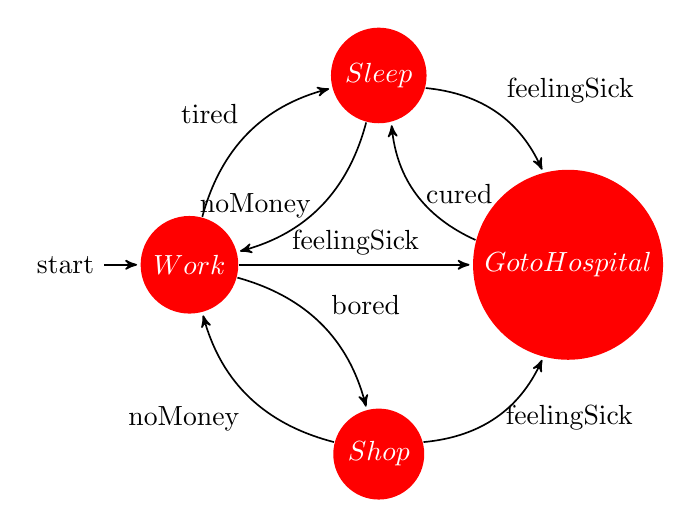
\begin{tikzpicture}[->,>=stealth',shorten >=1pt,auto,node distance=3.4cm,
                    semithick]
  \tikzstyle{every state}=[fill=red,draw=none,text=white]

  \node[initial,state] (A)                    		{$Work$};
  \node[state]         (B) [above right of=A] 	{$Sleep$};
  \node[state]         (E) [below right of=B]    	{$Go to Hospital$};
  \node[state]         (D) [below left of=E]		{$Shop$};
  
  \path (A) edge [bend left] node {tired} (B)
           (B) edge [bend left]  node[left] {noMoney} (A)
        	(B) edge [bend left] node {feelingSick} (E)
        	(A) edge [bend left] node {bored} (D)
        	(D) edge [bend left] node {noMoney} (A)
        	(E) edge [bend left] node [right] {cured} (B)
        	(A) edge node {feelingSick} (E)
        	(D) edge [bend right] node [right] {feelingSick} (E)
          ;
\end{tikzpicture}
\caption{Example for Agent behaviour modeled as a finite state machine}
\label{fig:statemachine}
\end{figure}

The common way to model agent behaviour is and has been using a finite state machine or other state-driven design approaches (for example a decision tree, as used in Unreal Engine 4 \footnote{\url{docs.unrealengine.com/latest/INT/Engine/AI/BehaviorTrees/}}). It is used in most agent-based simulations (for example \cite{biowar}) or games \cite{states}.

Fig.\ref{fig:statemachine} depicts such a model, displayed as a graph. Hereby nodes resemble a certain state, e.g. an action the agent does, for example work at his office. These states can also have sub-states, further specifying behaviour. For example, the \textit{Work} state may have the sub states \textit{Go to Workplace}, \textit{Do Work}, \textit{Eat at the Canteen} or \textit{Drink Coffee}. These may also be modeled as a finite state machine (with further sub-states) or use a stack.

Edges in the graph are associated with a certain condition the agent or environment must fulfill to transfer to another state. In our example, the agent would adopt the \textit{GotoHospital} state as soon as he feels sick.

But contrary to the common approach, our agent model doesn't make use of a state-based design. Rather, we decided to use a rule-based approach, which we will descripe in the next chapter.

Our reasoning for this decision is as follows: Finite state machines have a lot of benefits. They are easy to implement and expand, can be understood fast and are simple to represented in a comprehensible manner. But they also force a lot of the decisions onto the designer, since every state has to be created by hand, as well as transitions and transition triggers. Especially in a simulation background, this could distort the insights gained by observing the application.

It is obvious that the designer of such a simulation is not able to model every coherence, especially since most of the time the goal of such an application is to grasp these connections themselves. This may lead to warping the parameters so it fulfills a certain goal, for example satisfying a preexisting statistic. Also, it may strive for huge amounts of empirical data (see: \cite{biowar}) since the inner workings of the model aren't based on emergence, but hard-coded procedures. 

\subsubsection{Agent Decision Making}
\label{sec:decisions}

Our model is based on the aspect of self-learning and keeping predefined routines to a minimum. To achieve these goals, we tried to develop a system based on the most basic motivators, reward and boredom. The idea for this approach is taken from \cite{adams}. In this science fiction story the author describes a robot working from the following paradigm:
Reward encourages the agent to find the most benefiting actions possible, while boredom prevents him from doing the same action all the time.

As a result of this approach, agent payoff $p_t$ (the general measurement for `well-doing' of an agent) at time $t$ is based only on the reward $r_t$ and boredom $b_t$, where $L(x)$ is the logistic function $\frac{1}{1 + e^{-12(x - 0.5)}}$:

\begin{equation*}
p_t := L(\frac{r_t (1 - b_t) - r_{t-1}(1-b_{t-1}) + 1}2)
\end{equation*}

The key drive for every agent is to maximize their payoff. Logistic scaling was applied to increase the impact of small improvements and prevent local maxima from dominating the learning process.

All other motivators, like hunger, social needs or health are secondary and part of the model only by influencing reward in one or another way. For example, in our simulation every agent has an attribute called wealth. It increases when she goes to work and decreases at the shop and the hospital. Current wealth or wealth gain isn't calculated into the reward parameter, but since it's mandatory to do rewarding activities like shopping, the agent includes working into his daily routine.

The same is true for infection. Diseases lower the reward of most actions, since working, drinking or shopping isn't much fun if the agent feels sick. To lower the risk of infection, agents stay at home more often to lower infection risk and visit the hospital more often. Also, this wasn't programmed into the agent model explicitly, but emerges from the inner logic of our learning model.

The base algorithm is an implementation of the Extended Classifier System (XCS) \cite{wilson1995classifier}. Since this learning system is far too complex to describe fully in this article, we will only explain the basic idea. The classifier system maps certain states of the agent and his surroundings to an action and weights them with an excepted payoff. Then the system selects the most promising action for the current state and execute it. The insights gained by performing the action will then feed back into the model to further improve the payoff estimation, applying an offset to motivate long term planning.

\begin{figure}[h]
\begin{subfigure}{0.5\textwidth}
\begin{equation*}
\text{State} = (r = 0.7, b = 0.2, w = 0, s = false)
\end{equation*}
\caption{Example of an agent state}
\end{subfigure}

\begin{subfigure}{0.5\textwidth}
\begin{center}
\begin{tabular}{c c c c|c c}
$r$ 		& $b$ 		& $w$		& $s$ 		& action & payoff 	\\ \hline 
$\leq0.5$	& $> 0.5$	& $> 0.5$	& $false$	& \textit{sleep}	&	0.2		\\
$\leq0.5$	& $\leq 0.5$	& $\leq 0.5$	& $true$	& \textit{work}	&	0.4		\\
$>0.5$	& $> 0.1$	& $= 0$	& $false$	& \textit{drink}	&	0.2		\\
$\leq0.8$	& $\leq 0.2$	& $= 0$	& $false$	& \textit{work}	&	0.8		\\
$\leq0.2$	& $> 0.8$	& $\leq 0.5$	& $true$	& \textit{sleep}	&	0.4		\\
$>0.2$	& $\leq 0.8$	& $\leq 0.2$	& $false$	& \textit{shop}	&	0.2		\\
\end{tabular}
\end{center}
\caption{An example ruleset}
\end{subfigure}

\begin{subfigure}{0.5\textwidth}
\begin{center}
\rowcolors{4}{green}{green}
\begin{tabular}{c c c c|c c}
$r$ 					& $b$ 					& $w$				& $s$ 		& action & payoff 	\\ \hline 
\cellcolor{orange}$ \leq0.5$	&  \cellcolor{orange} $> 0.5$	&\cellcolor{orange} $> 0.5$	& $false$	& \textit{sleep}	&	0.2		\\
\cellcolor{orange}$\leq0.5$	& $\leq 0.5$	& $\leq 0.5$	& \cellcolor{orange}$true$	& \textit{work}	&	0.4		\\
$>0.5$	& $> 0.1$	& $= 0$	& $false$	& \textit{drink}	&	0.2		\\
$\leq0.8$	& $\leq 0.2$	& $= 0$	& $false$	& \textit{work}	&	0.8		\\
\hiderowcolors
$\cellcolor{orange}\leq0.2$	&\cellcolor{orange} $> 0.8$	& $\leq 0.5$	& \cellcolor{orange}$true$	& \textit{sleep}	&	0.4		\\ \showrowcolors
$>0.2$	& $\leq 0.8$	& $\leq 0.2$	& $false$	& \textit{shop}	&	0.2		\\
\end{tabular}
\end{center}
\caption{Rules that fulfill the state}
\end{subfigure}

\begin{subfigure}{0.5\textwidth}
\begin{center}
\rowcolors{3}{green}{white}
\begin{tabular}{c c c c|c c}
$r$ 		& $b$ 		& $w$		& $s$ 		& action & payoff 	\\ \hline 
$>0.5$	& $> 0.1$	& $= 0$	& $false$	& \textit{drink}	&	0.2		\\
$\leq0.8$	& $\leq 0.2$	& $= 0$	& $false$	& \textit{work}	&	0.8		\\
$>0.2$	& $\leq 0.8$	& $\leq 0.2$	& $false$	& \textit{shop}	&	0.2		\\
\end{tabular}
\end{center}
\caption{Selected rule according to highest payoff}
\end{subfigure}
\caption{Sample for agent decision making}
\label{fig:xcs}
\end{figure}

Fig. \ref{fig:xcs} shows an example for agent decision making. The agent state $S :=(r,b,w,s)$ describes the current state of the agent, where $r$ is the current reward value, $b$ the boredom, $w$ the wealth and $s$ as an indicator whether the agent is feeling sick/ is infected. While the ruleset for each agent is calculated before the simulation to limit processing power needed, the weights of the different rules are updated every step.

\subsubsection{Agent Actions}

When the agent has decided which action to take, he has one of five possibilities: Sleep at a house, work at an office,  shop at a mall or go to the hospital. Each action consists of the following pattern:
\begin{enumerate}
\item Go to the desired place
\item Execute the action, gaining or loosing reward and boredom
\item Reevaluate the state, decide on a new action
\end{enumerate}

The agent will always go to the nearest building that provides a opportunity for the desired action. The agents aren't bound to a specific home or office, which could be a feature for later iterations of the simulation. If the path to all of the mandatory buildings are blocked, the agent will perform an \textit{idle} action for some time, doing nothing and increasing boredom in the process.

Each action will change the agent state. For example, working at an office will increase wealth as well as boredom. Going shopping or drinking will increase reward, but only if the agent can provide enough wealth to pay for these actions, which is decreased in the process. If she can't, only boredom is increased as a penalty.

Also, long travel distances are penalized with increased boredom. This helps the agent to favor optimized travel routes and daily routines and will also punish the user for providing bad infrastructure, since he has to keep both the happiness and health of the agents at high levels.

The sole purpose of this advanced agent model is to provide advanced agents to the simulation, which can adapt to situation the user and environment provide through changing infrastructure. The inner workings of decision making as well as the state values of each agent are concealed from the user. Solely the \textit{happiness} value as the mean value over reward and boredom gives feedback about how well the created infrastructure is supporting the needs of its inhabitants.

\subsection{Learning Goals}

With this interactive simulation, the user should be able to learn the inner workings of an epidemic outbreak. We emphasized a lot on the intertwining aspects of infrastructure and disease spread.

This manifests in setting the goal for the user to keeping the infection in check while keeping the infrastructure in tact. Hence providing access to all vital buildings in a community is also a vital aspect to consider. The user shall grasp that often keeping support in the community for his actions is at least as important as separating the ill from the healthy.
For example, in the case of the Ebola outbreak, language barriers, fear and misinformation played a vital part in the treatment of the epidemic\footnote{\url{www.newscientist.com/article/mg22329774.600-fighting-fear-denial-and-death-on-ebola-frontline}}. 

Of course, this simulation can't display all important factors involved. But by focusing on the underlying systems rather than specific manifestations of the problem, we hope the user is able to transfer the learned knowledge onto all kinds of situations.

\section{Project Requirements}

In the following section, each of the requirements that was challenged towards the project is highlighted subsequently. It will be emphasized how the simulation keeps the user engaged without compromising on scientific relevance. Also, it will be outlined how reduction of perceived complexity and the aesthetics used help to make the user understand the insights and mechanics of the model while keeping her from being overwhelmed. 

\subsection{Science}
%\begin{itemize}
%\item CoSMoS compliant
%\item validity
%\item innovation
%\item scientific context
%\item exploration value
%\item model representation
%\end{itemize}

The underlying model has potential for lots of scientific insight. As we stated before, we don't try to emulate a specific real-world scenario. Thus, we renounce to use empirical data but rather rely on a more complex and emergent model design.

Our model takes multiple factors of disease spread into account: Social interactions between agents (going into a shop or office together), various factors of infrastructure (spatial and temporal separation, route-finding) as well as different means of infection (direct contact, over air, with and without delayed incubation time). These all are grounded on real-world factors, but rather than designing most of these by hand, the model itself devises these aspects out of its inner logic.

Our ambitious and self-learning agent model makes it possible to create a system that models these factors without being to dependent on design decisions. In the contrary, its emergence emphasizes the underlying system of epidemics rather than their concrete manifestations. 

We believe that this level of abstraction is vital to gaining insight of the inner workings of such a complex entity as is a epidemic and its various social and structural facets.
This focus on mechanics rather than the concrete result is the novel approach that makes our simulation stand out from existing approaches like Biowar.

\subsection{Gamification}
%\begin{itemize}
%\item interaction possibilities
%\item interaction guidance
%\item game elements
%\item relatedness
%\item competence
%\item autonomy
%\end{itemize}

Our simulation features lots of different features that support gamification. Gamification supports us in the strive for a comprehensible and captivating experience that makes learning and understanding the principles of disease spread rather a treat than a threat.

We implemented gamification on every level of the application. We designed an interface that rater supports the feeling that you're playing a game than exploring a scientific model. Also, our means of input include various forms of game-pads,  with focus on the XBox 360 / One controller.

At last, the procedure of the simulation itself creates the impression of a game, featuring multiple levels, a goal that has to be reached and penalties for not understanding the mechanics of the model (a \textit{lose} condition if the epidemic isn't kept in check). 

By directly aligning the `game' goals (saving the city from plague spread) and the learning goals (understanding which infrastructural aspects like containment influence disease spread) with each other, our implementation of gamification supports solely the purpose of scientific insight. This way, we prohibit the gaming aspect to take over and warp the scientific model just to increase excitement and appeal.

\subsection{Complexity}
%\begin{itemize}
%\item learning processes
%\item conveyed complexity
%\item model complexity
%\item real-time methods
%\end{itemize}

The presented interactive simulation features great complexity in it's inner workings, due to the emergent nature of self-learning, multi-agent based models as used in our model. Also, additional complexity is added by the intertwining aspects of the infrastructural network and its changing nature based on user input.

Much of these complexity is omitted from the user experience. For example, the complex decision making process is only recognizable by the agents actions, which are also simplified, since the whole set of citizens is perceived as one entity by the user.

Also, some of the inner workings of the model can't be noticed at all. The wealth value as well as the exact composition of the happiness value have no representation in the user interface. This decision was made consciously since providing the user with too much information may prove counterproductive in achieving the learning goals.

Consequences of actions the user invokes are only observed through their top-level results, like changes in the most frequent used streets or the general happiness value. Through the iterating nature of the level design, the inner mechanics of the model can be understood a little bit better with each new challenge.

\subsection{Aesthetics}

Our main goal concerning aesthetics was to generate a comprehensible, easy-to-understand user experience. Thus we focused on providing an abstract and simple user interface to not distract from the core statements of our simulation.

Since our model is mainly about infrastructure, the user must be able to understand the various emergent features as well as the interaction of micro and macro levels inside our simulation. Graphics had to be displayed in a fashion that can be understood without much explanation or interpretation while keeping as much abstraction as possible.

Therefore, we decided that a top down view would provide the best suited presentation of the various interactions happening in our model. To keep in line with the goal of simplicity, we decided to use graphics in an ``8-bit like'' style, used in games of the SNES era or in recent releases of the Indie-game scene, like \textit{Binding of Isaac}, \textit{Faster than Light}, \textit{Hotline Miami} or \textit{Dungeon of the Endless}.
 
This type of graphics yields multiple benefits, hence it's rapid increase in popularity over the recent years. It is easy to comprehend for the user, since it uses simple assets and reduces distracting visual effects like advanced lighting or complex animations to a minimum. Because of this features, it's also easy to use and implement by the designer, providing time and focus for the more complex and important aspects of the simulation.

\newpage

\section{Summary \& Future Work}
%\begin{itemize}
%\item summarise your work (motivation, concept, implementation, fulfilment of the requirements)
%\item describe what you would like to do next in the context of the presented work
%\item why is the presented work a good starting point for these ideas?
%\item where would be the benefit of the outlined future work?
%\end{itemize}

We provided an interactive simulation that is both exciting and insightful for the user to explore. Using abstraction were applicable, a complex agent model and an easy to comprehend display of a simulated city, we created a model representation that is easy to comprehend but complex in its inner mechanics.

Both the emergence of epidemics and infrastructure based on social and spatial factors was accommodated by our model. Inclusion of win and lose conditions, game-pad support and other game-like features help to keep the user engaged.

Due to time restrictions, it was not possible to implement all features as exhaustive as the complexity of the matter demands.

In case of the agent model, there are lots of factors not accounted for. For example, inter-human relationships, like families, social networks or segregated communities, could be implemented.

Also, the self-learning aspect could be improved greatly. While agents extract knowledge from their current situation, the means of adaptation are limited. For example, agents could avoid quarantine-zones by themselves, spread knowledge through others or create communities. Furthermore, it's still hard to see and comprehend these self-learning capabilities in the simulation.

Concerning the infrastructure aspect, our approach is as simple as it gets. Neither time of day differences, public transportation nor complex layouts of streets or any other advanced manifestation of traffic are part of the model. Also, agents aren't bound to a specific home or workplace, like they would be in real life. 

An idea for further work would be to merge this simulation with an advanced traffic system, for example the model used in the game \textit{Cities: Skylines}\footnote{\url{www.citiesskylines.com}}.The simulation could then be implemented as an in-game modification.



\bibliographystyle{alpha}
\bibliography{sciwri}  

\end{document}
